\section{Results}
\label{sec:results}
\subsection{User Experience}
\label{sec:ux}

Before setting up and using the Safeplug device, we read a variety of news articles as well as opinions through the Tor mailing list~\cite{tormailinglist}.  There were many thoughts on the Terms of Service and the option to use the device as a Tor relay node; this inspired us to start our analysis with these items.  

\subsubsection{Terms of Service}
Safeplug's Terms of Service are interesting because they are controlling, yet the product they are for is a device for anonymization.  The first section of the Terms of Service explains how to agree to them:

\begin{quotation}
``You must agree to these TOS before you can use the Service. You can agree to these TOS by: a) actually using the Service, or b) clicking a box that indicates you agree to the Service, where such a box is made available to you.'' \cite{safeplug}
\end{quotation}

This is worth noting because option b) described above did not exist in any part of the setup process for Safeplug.  The Terms of Service continues by notifying readers that Pogoplug can change them any time they wish:

\begin{quotation}
``Pogoplug may update or change these TOS from time to time and recommends that you review the TOS on a regular basis at www.pogoplug.com/safeplug. You understand and agree that your continued use of the Service after the TOS has changed constitutes your acceptance of the TOS as revised. '' \cite{safeplug}
\end{quotation}

Most Safeplug users will likely not read the Terms of Service once, let alone on a regular basis; therefore, most users will be blind to any changes.  It is also interesting that these Terms of Service are only accessible through a small link at the bottom of the Safeplug website \cite{safeplug}; specifically, there is no documentation, including the Terms of Service, in the package that the device was shipped in.  Further along in the Terms of Service, the makers of Safeplug were sloppy when they wrote:

\begin{quotation}
``Pogoplug includes several open source components in the Software. You agree to abide by the terms of the relevant licenses, as may be updated by Pogoplug from time to time at http://pogoplug.com/home-en-developers-open-source.html. '' \cite{safeplug}
\end{quotation}

The link included is a dead link and takes the user to a web page with a 404 error.  This may indicate that there are other errors related to Safeplug (potential security vulnerabilities).  The last section of the Terms of Service that stood out described Pogoplug's policy on updates:

\begin{quotation}
``As part of the Service, you may from time to time receive updates to the Software from Pogoplug that may be automatically downloaded and installed to your applicable device. These updates may include bug fixes, security enhancements or improvements, or entirely new versions of the Software. You agree that Pogoplug may automatically deliver such updates to you as part of the Service. '' \cite{safeplug}
\end{quotation}

This should raise a red flag for users because they may not know when the software in their device is being changed or what it is changing to.  While Safeplug makes many claims about providing anonymity, users are simply putting their trust in a different entity, namely Pogoplug.

\subsubsection{Tor Relay Node Option}
One of Safeplug's configurations is the use of the device as a Tor relay node in the Tor network.  When the device is initially setup, the default setting is to not use it as a relay node.  

One of our concerns is how understandable this setting is to the average Internet user.  The settings page describes Tor in an extremely basic way, as shown in Figure~\ref{fig:funnydesc}, but describes the functionality of a Tor relay node in a much more technical manner.  This description is shown in Figure~\ref{fig:relaydesc}.  If the majority of users can only understand the simpler description, then they likely won't understand the description of a Tor relay node.  This could be a problem if users simply decide not to do anything with that setting (i.e. don't change the setting to use Safeplug as a relay node).  Then there would be a large increase in use of the Tor network, yet most of the users are not giving back to it.

\begin{figure}[htb]
\begin{center}
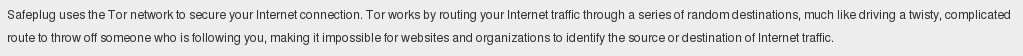
\includegraphics[width=\textwidth]{funnydesc.png}
\caption{This is a figure.}
\label{fig:funnydesc}
\end{center}
\end{figure}

\begin{figure}[htb]
\begin{center}
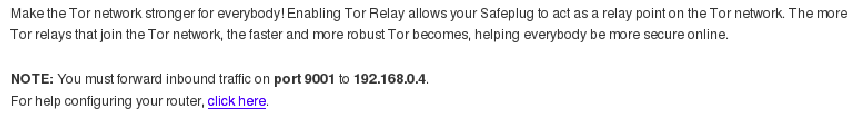
\includegraphics[width=\textwidth]{relaydesc.png}
\caption{This is a figure.}
\label{fig:relaydesc}
\end{center}
\end{figure}

This could easily be remedied; Safeplug should choose a target audience and have consistent descriptions.  The best option is to explain the Tor network and the functionality of a Tor relay node at the same level, preferably a level that normal Internet users can understand.  This increases the chances that users will run their Safeplug as a relay node.

\subsubsection{Internet Use}
    -Setting it up
    -Using the internet (show before and after for IP addresses)
    -Cookie experience First party cookies

\subsection{Teardown}
\label{sec:tear}

\subsubsection{Components}
    -Parts in the box

\begin{figure}[htb]
\begin{center}
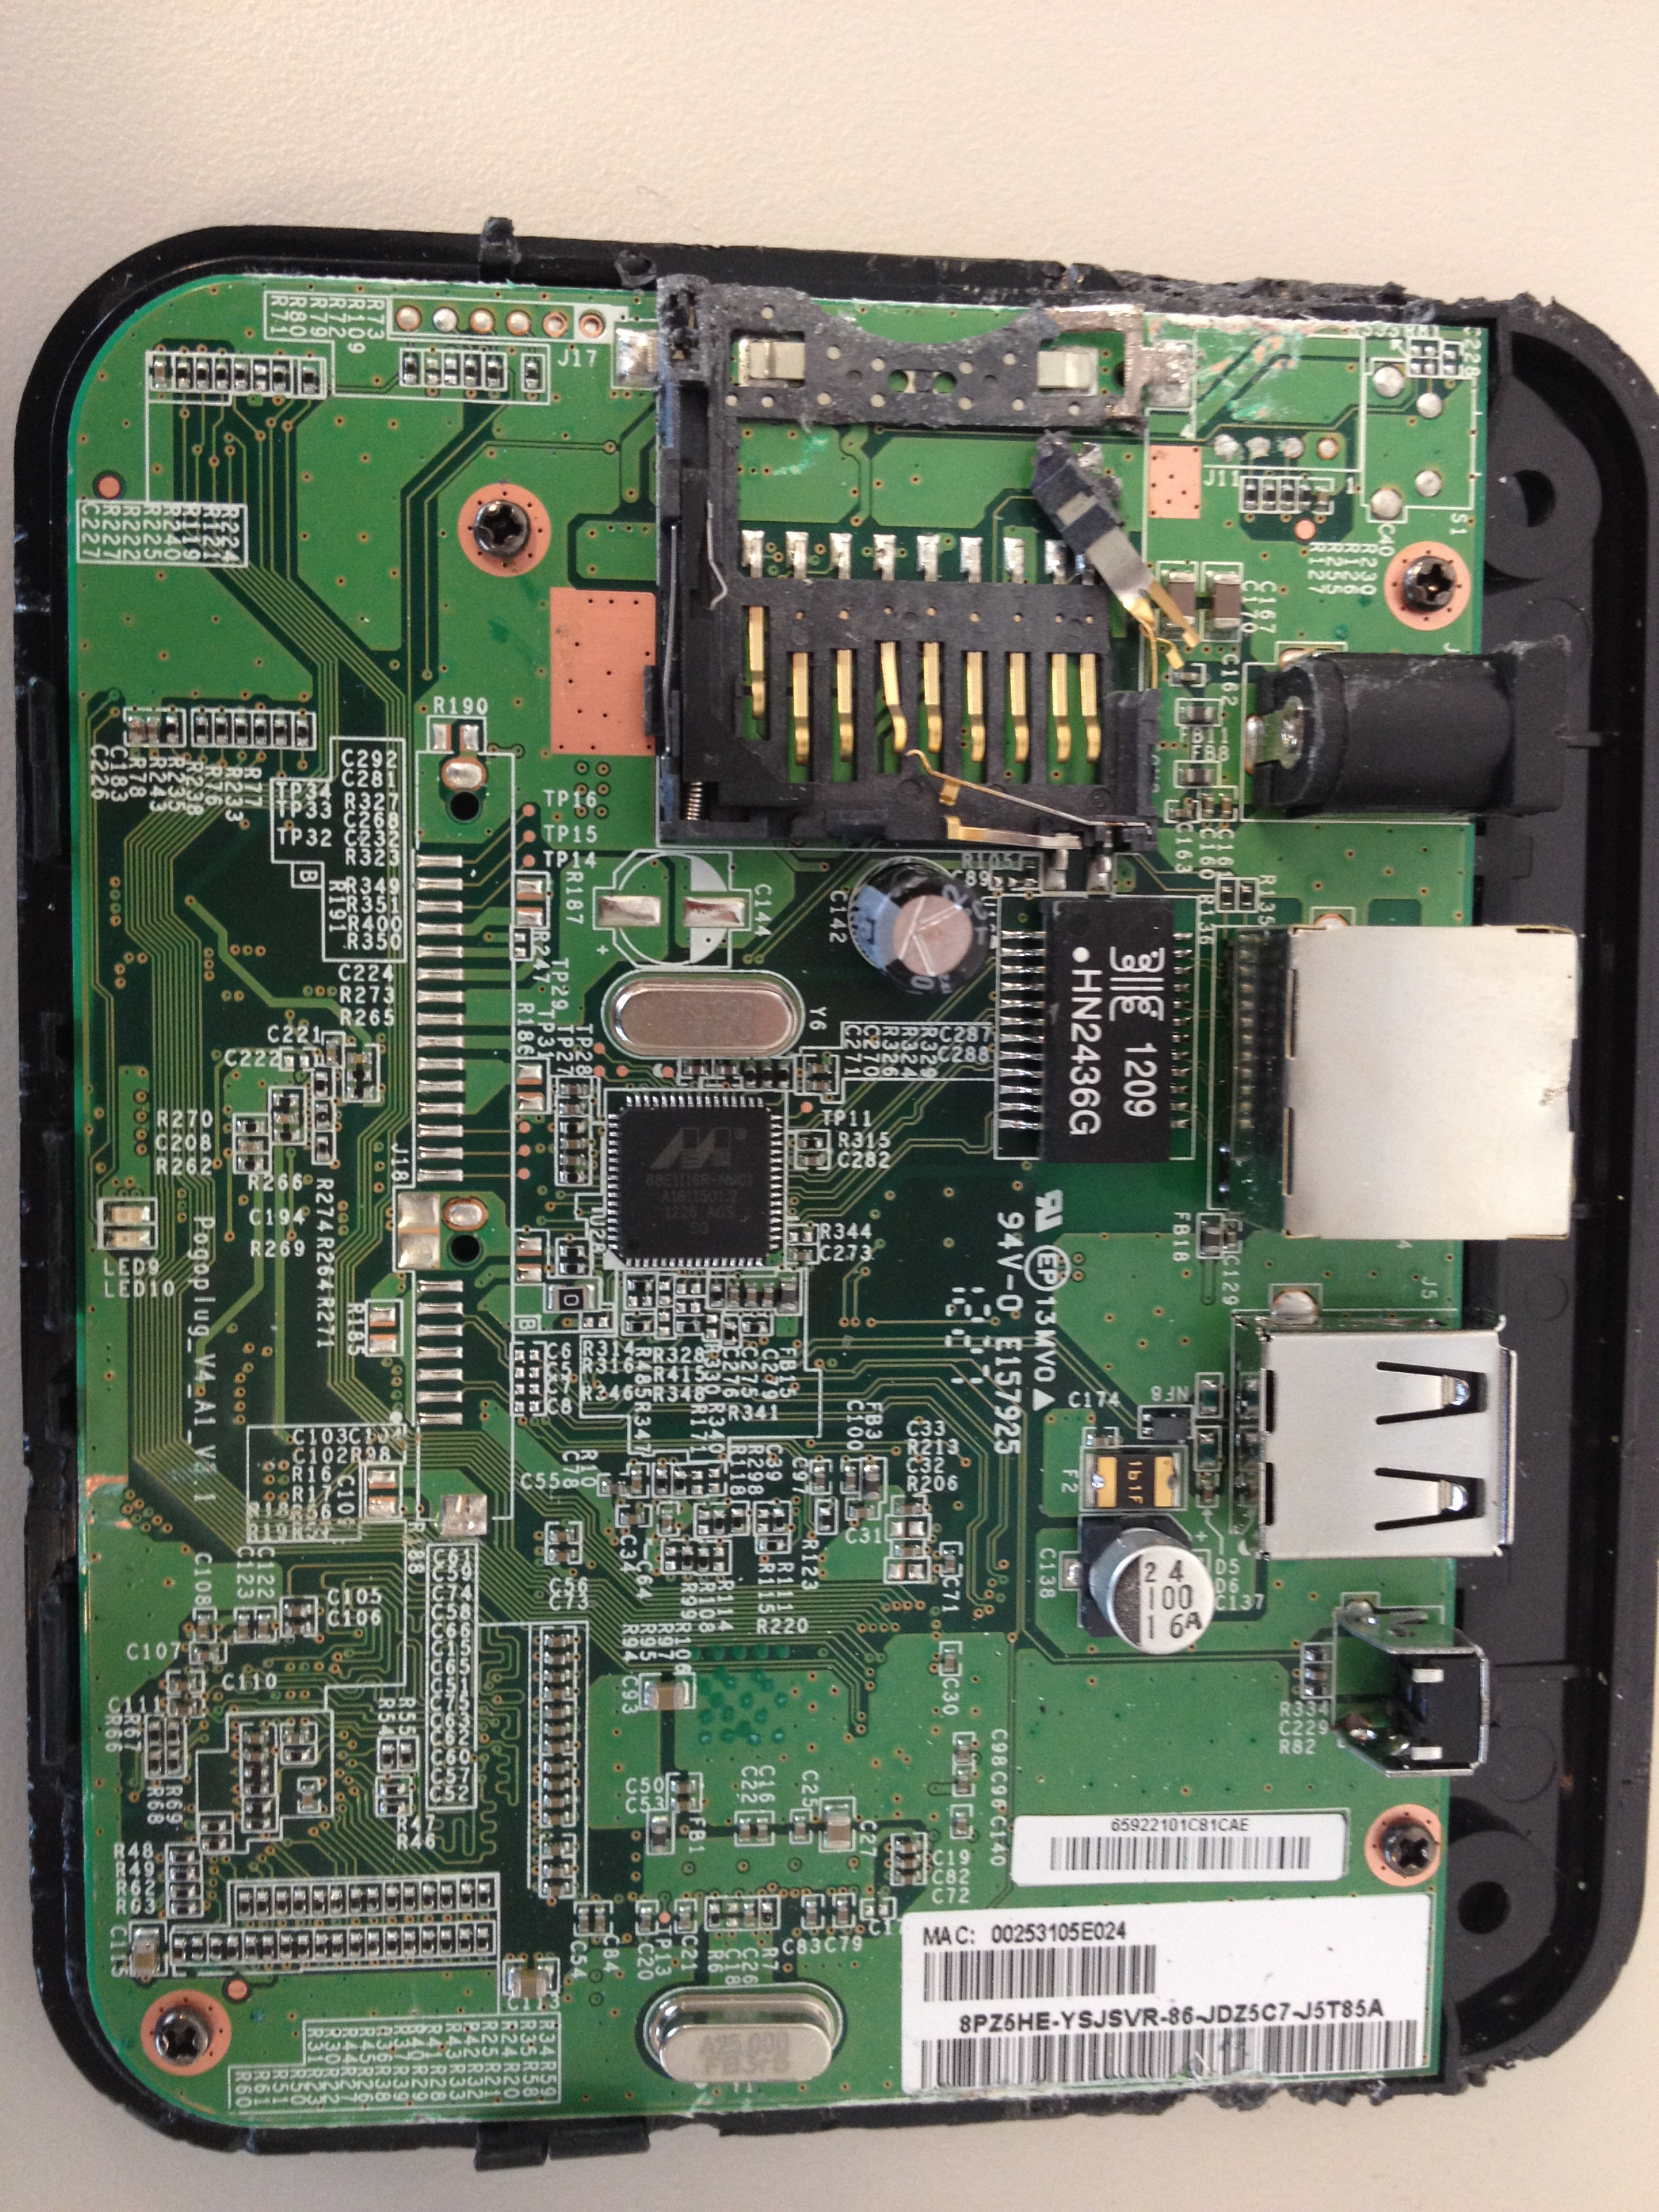
\includegraphics[width=0.25\textwidth]{safeplug_top}
\caption{This is a figure.}
\end{center}
\end{figure}

\begin{figure}[htb]
\begin{center}
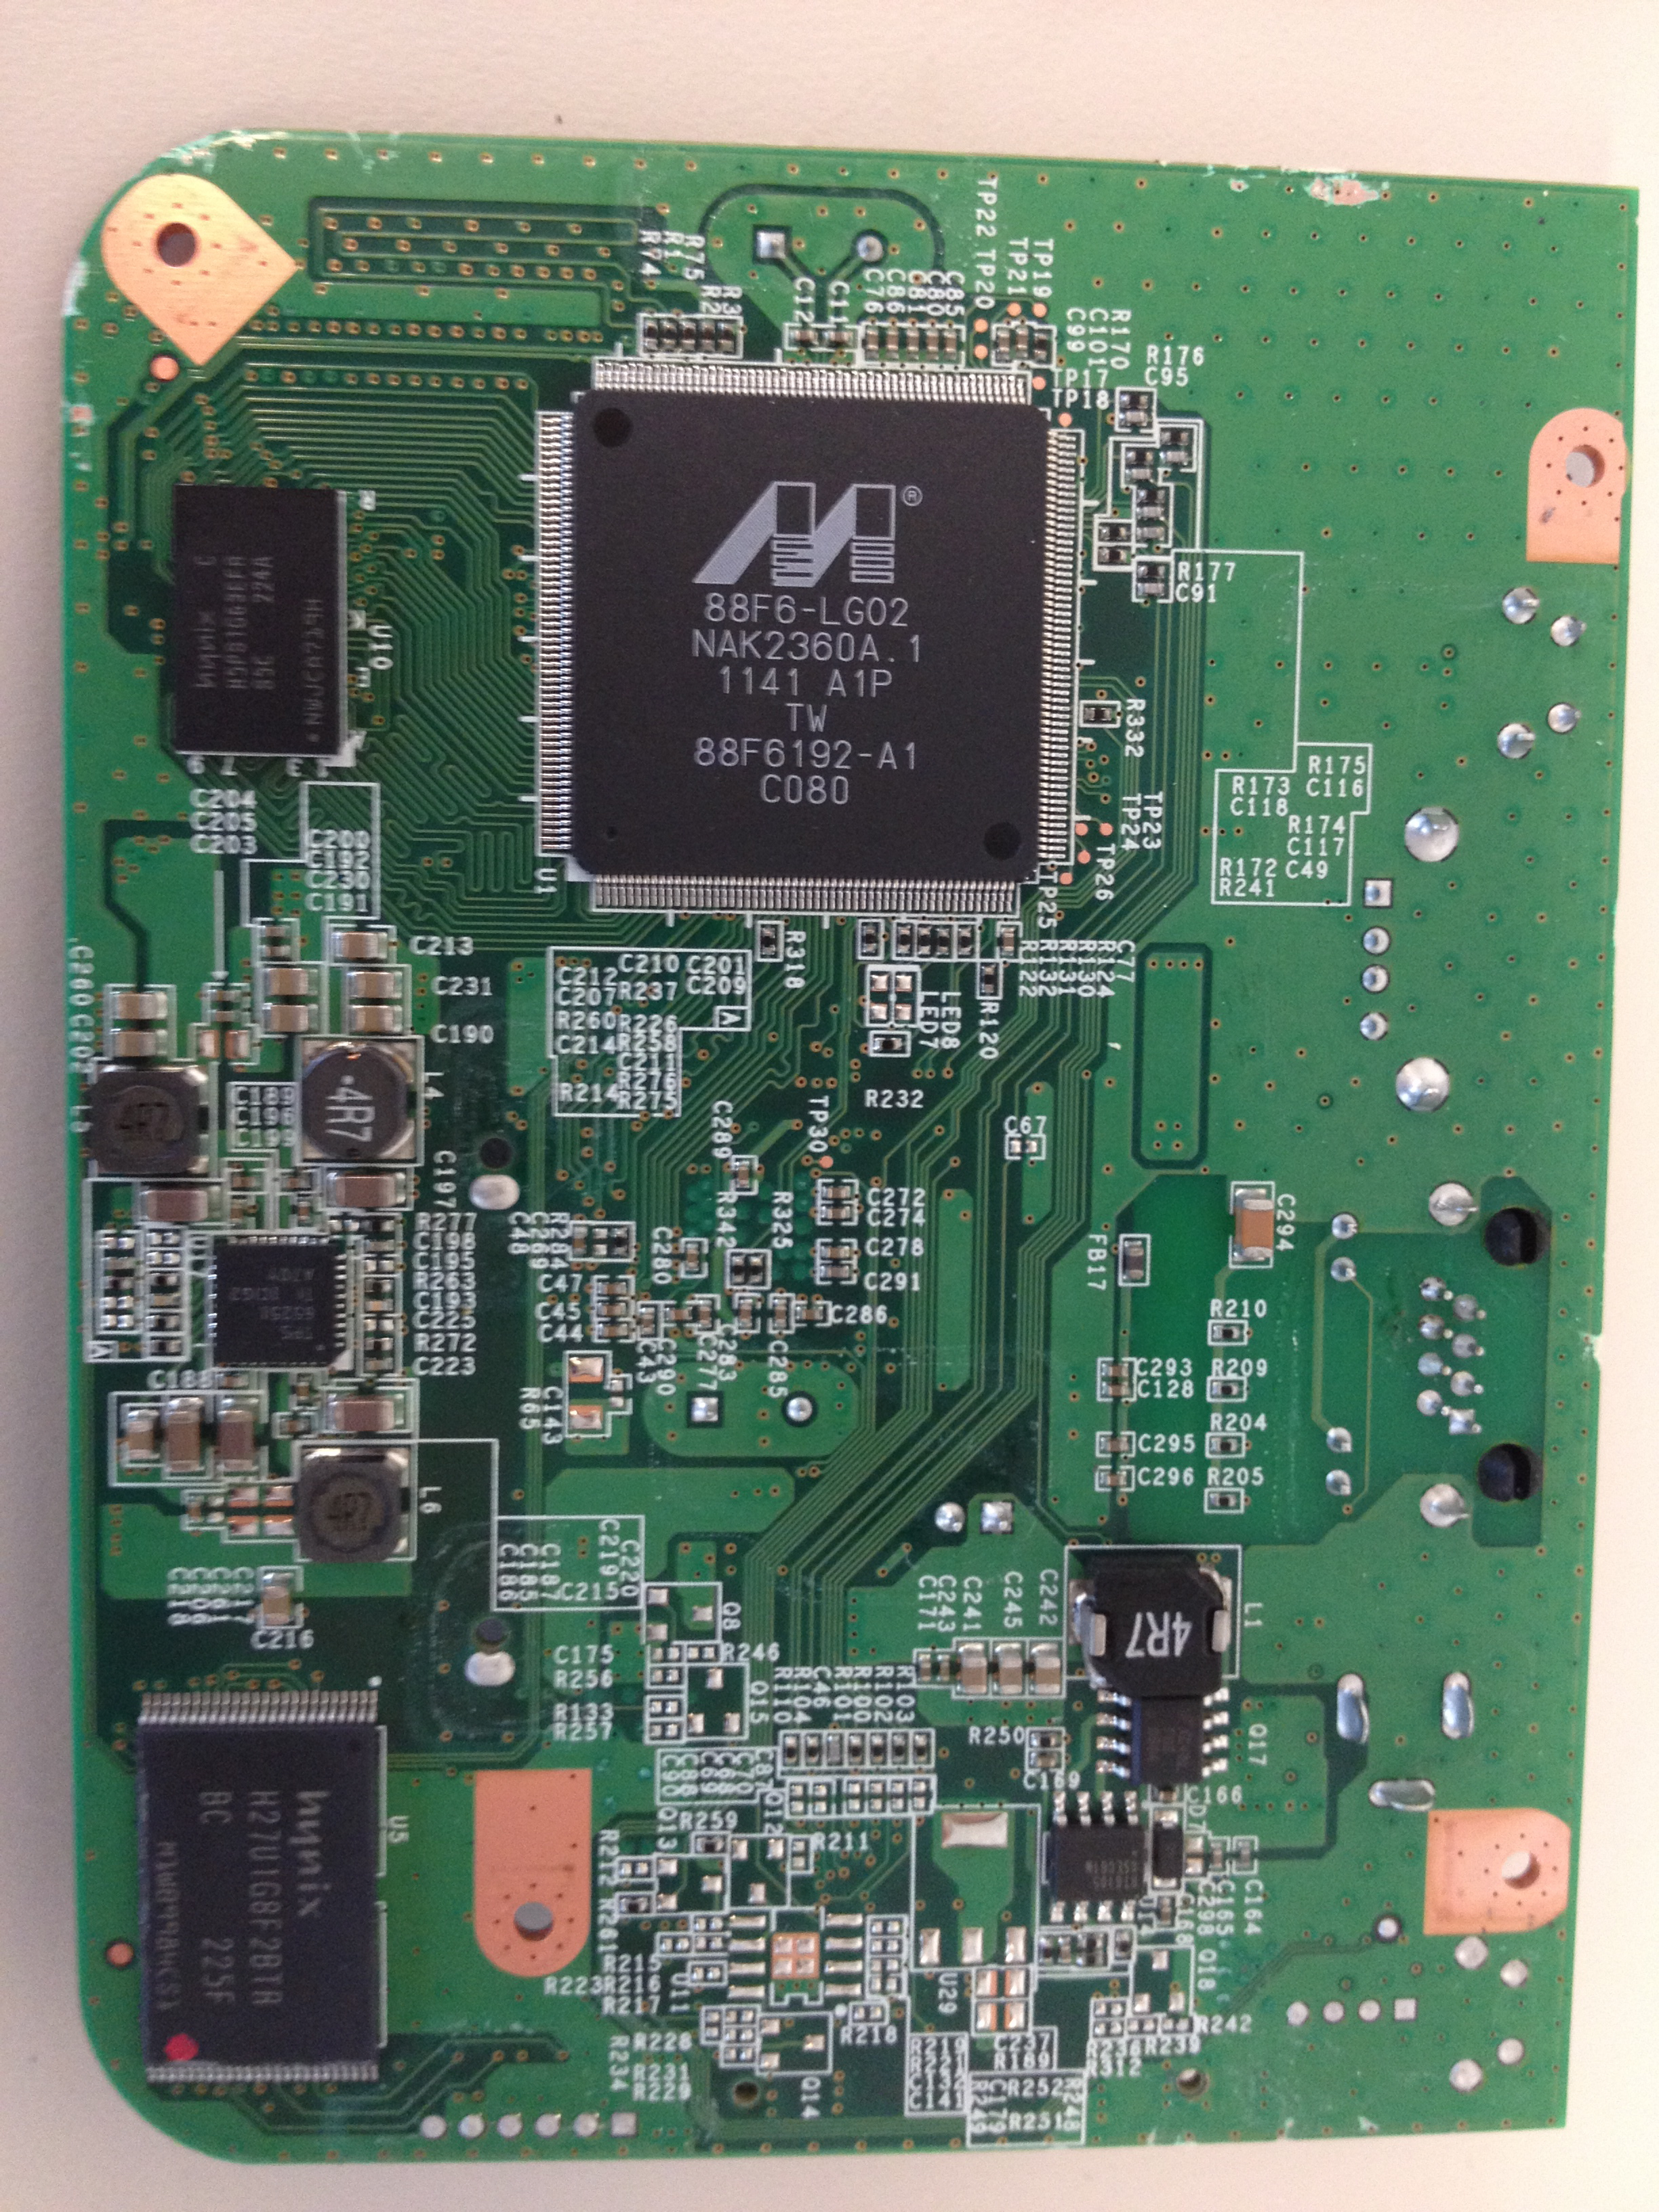
\includegraphics[width=0.25\textwidth]{safeplug_bottom}
\caption{This is a figure.}
\end{center}
\end{figure}

\subsubsection{Possible Attacks}
    -Possible attacks via USB/SD Card

